\chapter{PERSYARATAN SISTEM }

\label{chapter:PERSYARATAN SISTEM}

\section{Deskripsi Pengguna}
Target pengguna utama dari aplikasi Food AI Rescue (FAR) secara umum adalah seluruh entitas yang terlibat dalam ekosistem pengelolaan surplus makanan, rantai pasok logistik sosial, dan penerima manfaat di tingkat komunitas. Sistem ini memfasilitasi kolaborasi multi-pihak yang dirancang agar ramah pengguna (\textit{user-friendly}), baik bagi masyarakat awam, pelaku usaha, maupun tim manajerial. Untuk memetakan kebutuhan sistem, pengguna aplikasi ini didetailkan ke dalam segmentasi dan peran (\textit{role}) sebagai berikut:

% \subsection{Segmentasi Pengguna}

\begin{figure}[htbp]
    \centering
    \includegraphics[width=1\textwidth]{image/bab2/segmentasi.png}
    \caption{Segmentasi Pengguna Food AI Rescue}
    \label{fig:segmentasi}
\end{figure}

\begin{enumerate}
    \item \textbf{Donatur Individu}
    \begin{itemize}
        \item \textbf{Segmen/Profil}: Masyarakat perorangan atau pelaku usaha skala mikro yang memiliki kelebihan produksi makanan dalam jumlah kecil (skala rumah tangga).
        \item \textbf{Peranan dan Hak Akses Utama}: Memiliki hak untuk mengunggah data makanan surplus, memperbarui status ketersediaan (\textit{inventory}), serta melakukan serah terima secara langsung. Pada saat serah terima menggunakan fitur Janji Temu (COD), pengguna wajib memindai QR Code milik Penerima sebagai bukti distribusi yang sah. Selain itu, donatur memiliki akses untuk memantau Dasbor Dampak Sosial (SROI) yang memuat laporan total porsi terselamatkan dan estimasi pengurangan emisi jejak karbon (CO$_2$).
        \item \textbf{Hak Akses AI}: Memiliki akses ke fitur bawaan AI \textit{Quality Verification}. Sebelum donasi dipublikasikan, donatur wajib memindai foto makanan menggunakan kamera AI ini guna memastikan kelayakan fisik dan higienitas visual. Selain itu, donatur juga dapat memindai (\textit{scan}) bahan makanan untuk mendapatkan rekomendasi resep masakan dari sistem.
    \end{itemize}
    \item \textbf{Donatur Kelompok/Korporat (Mitra Penyedia)}
    \begin{itemize}
        \item \textbf{Segmen/Profil}: Pelaku bisnis skala besar di sektor \textit{Hospitality, Restaurant, and Cafe} (HORECA) seperti restoran, hotel, atau usaha katering berskala komersial.
        \item \textbf{Peranan dan Hak Akses Utama}: Memiliki peranan dan hak akses operasional yang sama persis dengan Donatur Individu, mulai dari siklus manajemen distribusi (unggah surplus, update \textit{inventory}, pindai QR serah terima) hingga pemantauan laporan di Dasbor Dampak Sosial (SROI).
        \item \textbf{Hak Akses Khusus (Spesial) AI}: Sebagai nilai tambah (\textit{value}) untuk mendukung kampanye pemasaran dan \textit{Corporate Social Responsibility} (CSR) perusahaan, donatur tingkat kelompok/korporat dibekali hak istimewa terhadap dua modul AI generatif eksklusif, yaitu:
        \begin{itemize}
            \item \textbf{\textit{Generate Image} Kemasan}: Hak spesial untuk menghasilkan gambar desain prototipe bungkus atau kemasan makanan.
            \item \textbf{\textit{Generate} Konten Media Sosial}: Hak spesial untuk secara otomatis menghasilkan gambar visual desain (lengkap dengan stiker verifikasi AI dan logo perusahaan) sekaligus memproduksi konten tulisan (\textit{copywriting}) promosi yang siap diunggah ke platform media sosial.
        \end{itemize}
    \end{itemize}
    \item \textbf{Penerima (Mitra Penerima)}
    \begin{itemize}
        \item \textbf{Segmen/Profil}: Masyarakat di kawasan rentan pangan, panti asuhan, dewan kemakmuran masjid (DKM), atau warga prasejahtera di desa sasaran yang membutuhkan bantuan makanan.
        \item \textbf{Peranan dan Hak Akses}: Memiliki akses untuk mencari menu makanan terdekat, melakukan proses klaim (\textit{booking}) guna mengunci stok dan mencegah insiden pengambilan ganda (\textit{double-claim}) oleh pihak lain, memilih metode pengambilan, dan menyajikan QR Code miliknya untuk dipindai saat makanan tiba.
        \item \textbf{Hak Akses Khusus AI}: Penerima diberikan akses ke fitur AI \textit{Quality Verification} untuk memindai kelayakan fisik dan higienitas visual makanan sebelum dikonsumsi, fitur \textit{Forum Request} untuk memublikasikan kebutuhan pangan spesifik, serta memberikan ulasan (\textit{feedback}).
    \end{itemize}
    \item \textbf{Relawan}
    \begin{itemize}
        \item \textbf{Segmen/Profil}: Pemuda lokal, warga desa, atau masyarakat umum yang bertindak secara sukarela (\textit{crowdsourcing}) sebagai armada logistik sosial.
        \item \textbf{Peranan dan Hak Akses}: Mengakses daftar misi pengantaran, melakukan penjemputan makanan dari lokasi Donatur, dan mengantarkannya secara langsung ke titik lokasi Penerima. Relawan memegang otoritas validasi lapangan dengan hak akses wajib pindai (\textit{mandatory scan}) QR Code milik Penerima sebagai syarat mutlak penyelesaian transaksi distribusi.
    \end{itemize}
    \item \textbf{Admin Pengelola}
    \begin{itemize}
        \item \textbf{Segmen/Profil}: Tim manajerial dan pengawas operasional harian yang bertugas mengelola sistem secara administratif di tingkat komunitas.
        \item \textbf{Peranan dan Hak Akses}: Memiliki hak akses dashboard admin untuk memverifikasi keabsahan pendaftaran akun baru secara manual, membekukan atau memblokir akun yang terbukti melakukan penyalahgunaan, menindaklanjuti laporan negatif, serta memantau Dasbor Statistik makro yang menampilkan peta panas (\textit{heatmap}) sebaran wilayah donasi dan kalkulasi SROI keseluruhan.
    \end{itemize}
    \item \textbf{Super Admin}
    \begin{itemize}
        \item \textbf{Segmen/Profil}: Pengembang sistem (Tim IT / \textit{Programmer}).
        \item \textbf{Peranan dan Hak Akses}: Memiliki tingkat hak akses paling tinggi dan menyeluruh pada sisi \textit{backend} aplikasi. Super Admin bertugas untuk melakukan pemeliharaan server secara berkala (\textit{maintenance}), menangani perbaikan apabila terdapat laporan \textit{bug} dari sistem, dan menjaga stabilitas basis data secara penuh.
    \end{itemize}
\end{enumerate}

\newpage

\section{Gambaran Sistem Saat Ini}
Gambaran sistem yang berjalan saat ini (\textit{As-Is}) pada ekosistem penyaluran donasi surplus makanan di masyarakat masih sepenuhnya mengandalkan metode konvensional secara manual dan tidak terstruktur. Hingga saat ini, belum ada satu pun aplikasi khusus atau sistem terintegrasi yang memfasilitasi tata kelola operasional logistik donasi pangan secara digital yang disertai dengan jaminan standar keamanan mutu. Startup JagoAI sebagai pihak inovator juga belum memiliki platform pusat kendali (\textit{command center}) untuk memonitor aktivitas donasi, memvalidasi kelayakan makanan secara otomatis, serta melacak pergerakan relawan kurir secara terpusat.
% \\
% Berdasarkan hasil observasi di lapangan, seluruh pencatatan data ketersediaan surplus makanan dan riwayat penyalurannya masih tidak terdokumentasi dengan baik atau hanya dicatat secara manual. Selain itu, proses pengecekan kelayakan dan keamanan pangan hanya mengandalkan observasi visual dengan mata telanjang oleh pihak donatur tanpa standar higienitas yang baku. Satu-satunya perangkat lunak yang umum digunakan dalam ekosistem penyaluran donasi saat ini hanyalah aplikasi pesan instan pihak ketiga (seperti grup WhatsApp), yang sekadar dimanfaatkan sebagai sarana komunikasi dasar, bukan sebagai sistem manajemen logistik terpadu maupun penyimpan basis data (\textit{database}). Ketiadaan sistem yang terintegrasi ini menyebabkan rantai informasi penjemputan sering terputus, tingginya risiko ancaman kesehatan bagi penerima akibat kelalaian manusia (\textit{human error}) dalam memvalidasi makanan, serta lambatnya proses distribusi yang berujung pada membusuknya makanan sebelum disalurkan sehingga tetap berakhir menjadi tumpukan limbah makanan (\textit{food waste}).
\subsection{Analisis Proses Bisnis}
Pada sistem manual, proses berbagi makanan berlebih berjalan secara sporadis, linear, dan tidak terstruktur. Ketika rumah tangga, penyelenggara acara, atau pelaku industri (seperti restoran dan hotel) memiliki surplus makanan, mereka harus mencari sendiri fasilitas sosial atau individu yang membutuhkan secara tatap muka atau melalui pesan singkat yang terbatas. Ketiadaan rantai pasok logistik yang terpusat ini menyebabkan waktu terbuang percuma hanya untuk mencari siapa yang bersedia menerima makanan tersebut. Akibatnya, banyak makanan yang awalnya masih layak konsumsi menjadi basi atau kedaluwarsa di tengah jalan, sehingga pada akhirnya tetap berujung dibuang ke Tempat Pembuangan Akhir (TPA) dan memicu masalah emisi gas rumah kaca.

\newpage
\begin{landscape}
    \centering
    \vfill
    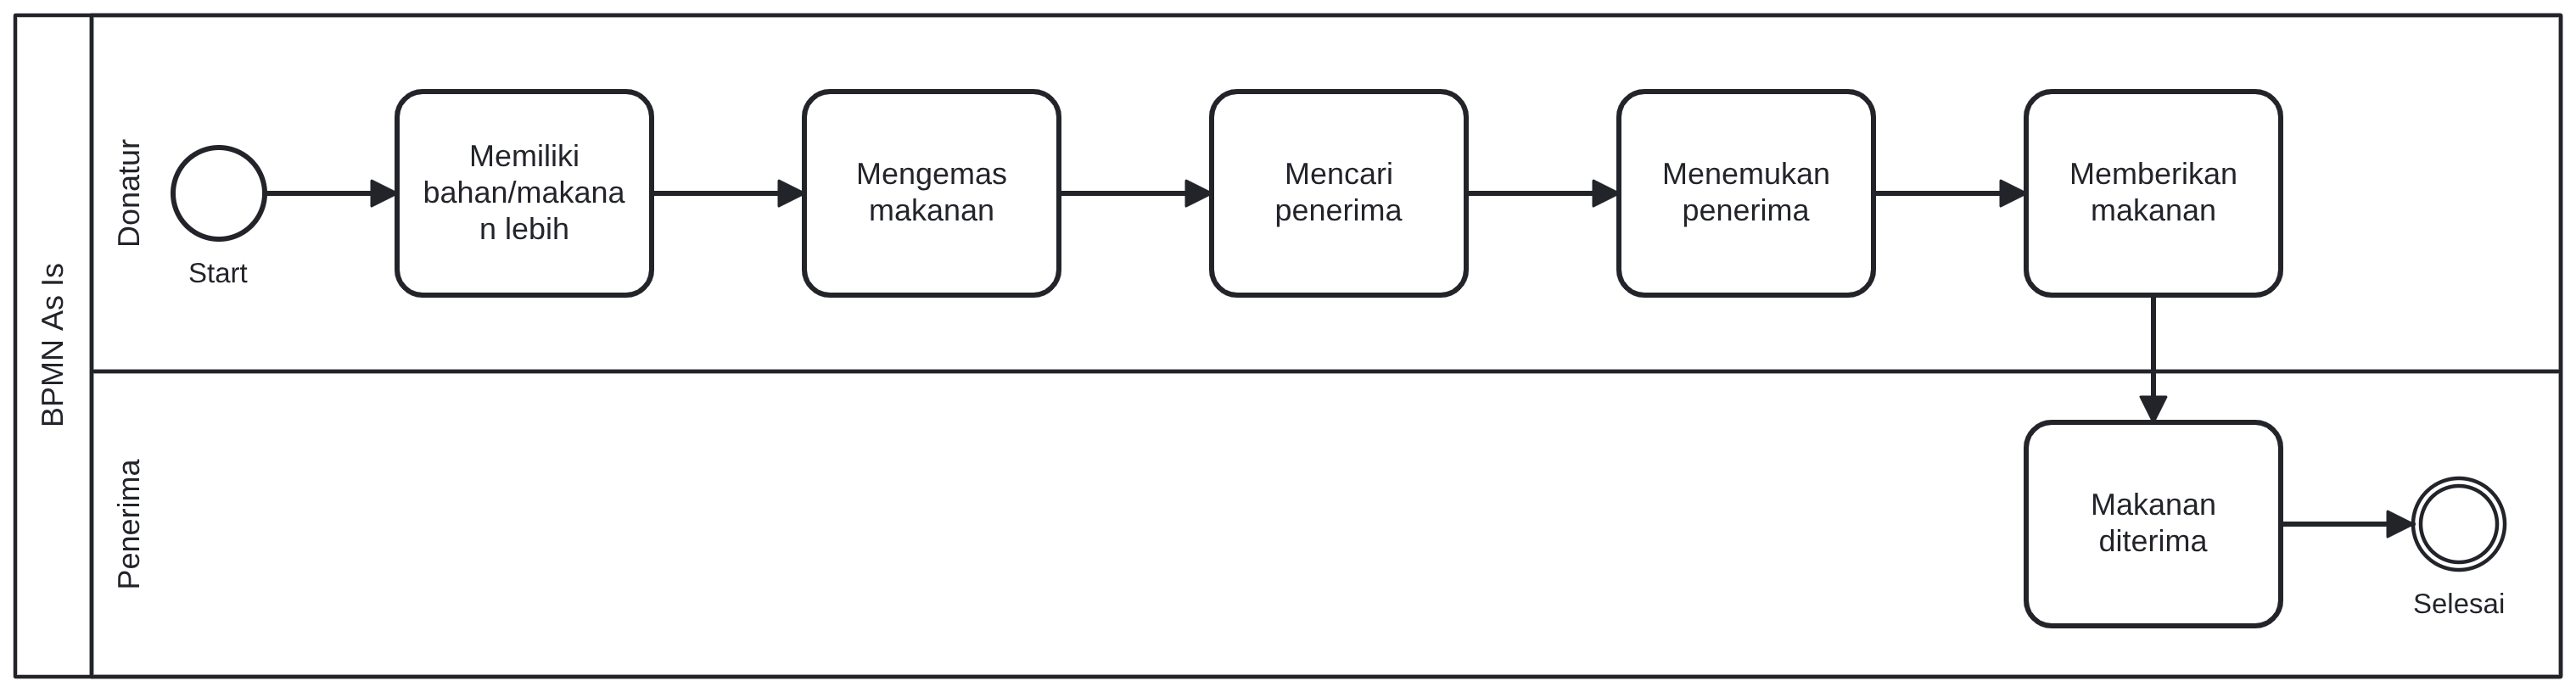
\includegraphics[width=0.9\linewidth]{image/bpmnAsIs.png}
    \captionof{figure}{Proses Bisnis Sistem Saat Ini (BPMN As-Is)}
    \label{fig:bpmnAsIs}
    \vfill
\end{landscape}

\newpage
\begin{landscape}
    \centering
    \vfill
    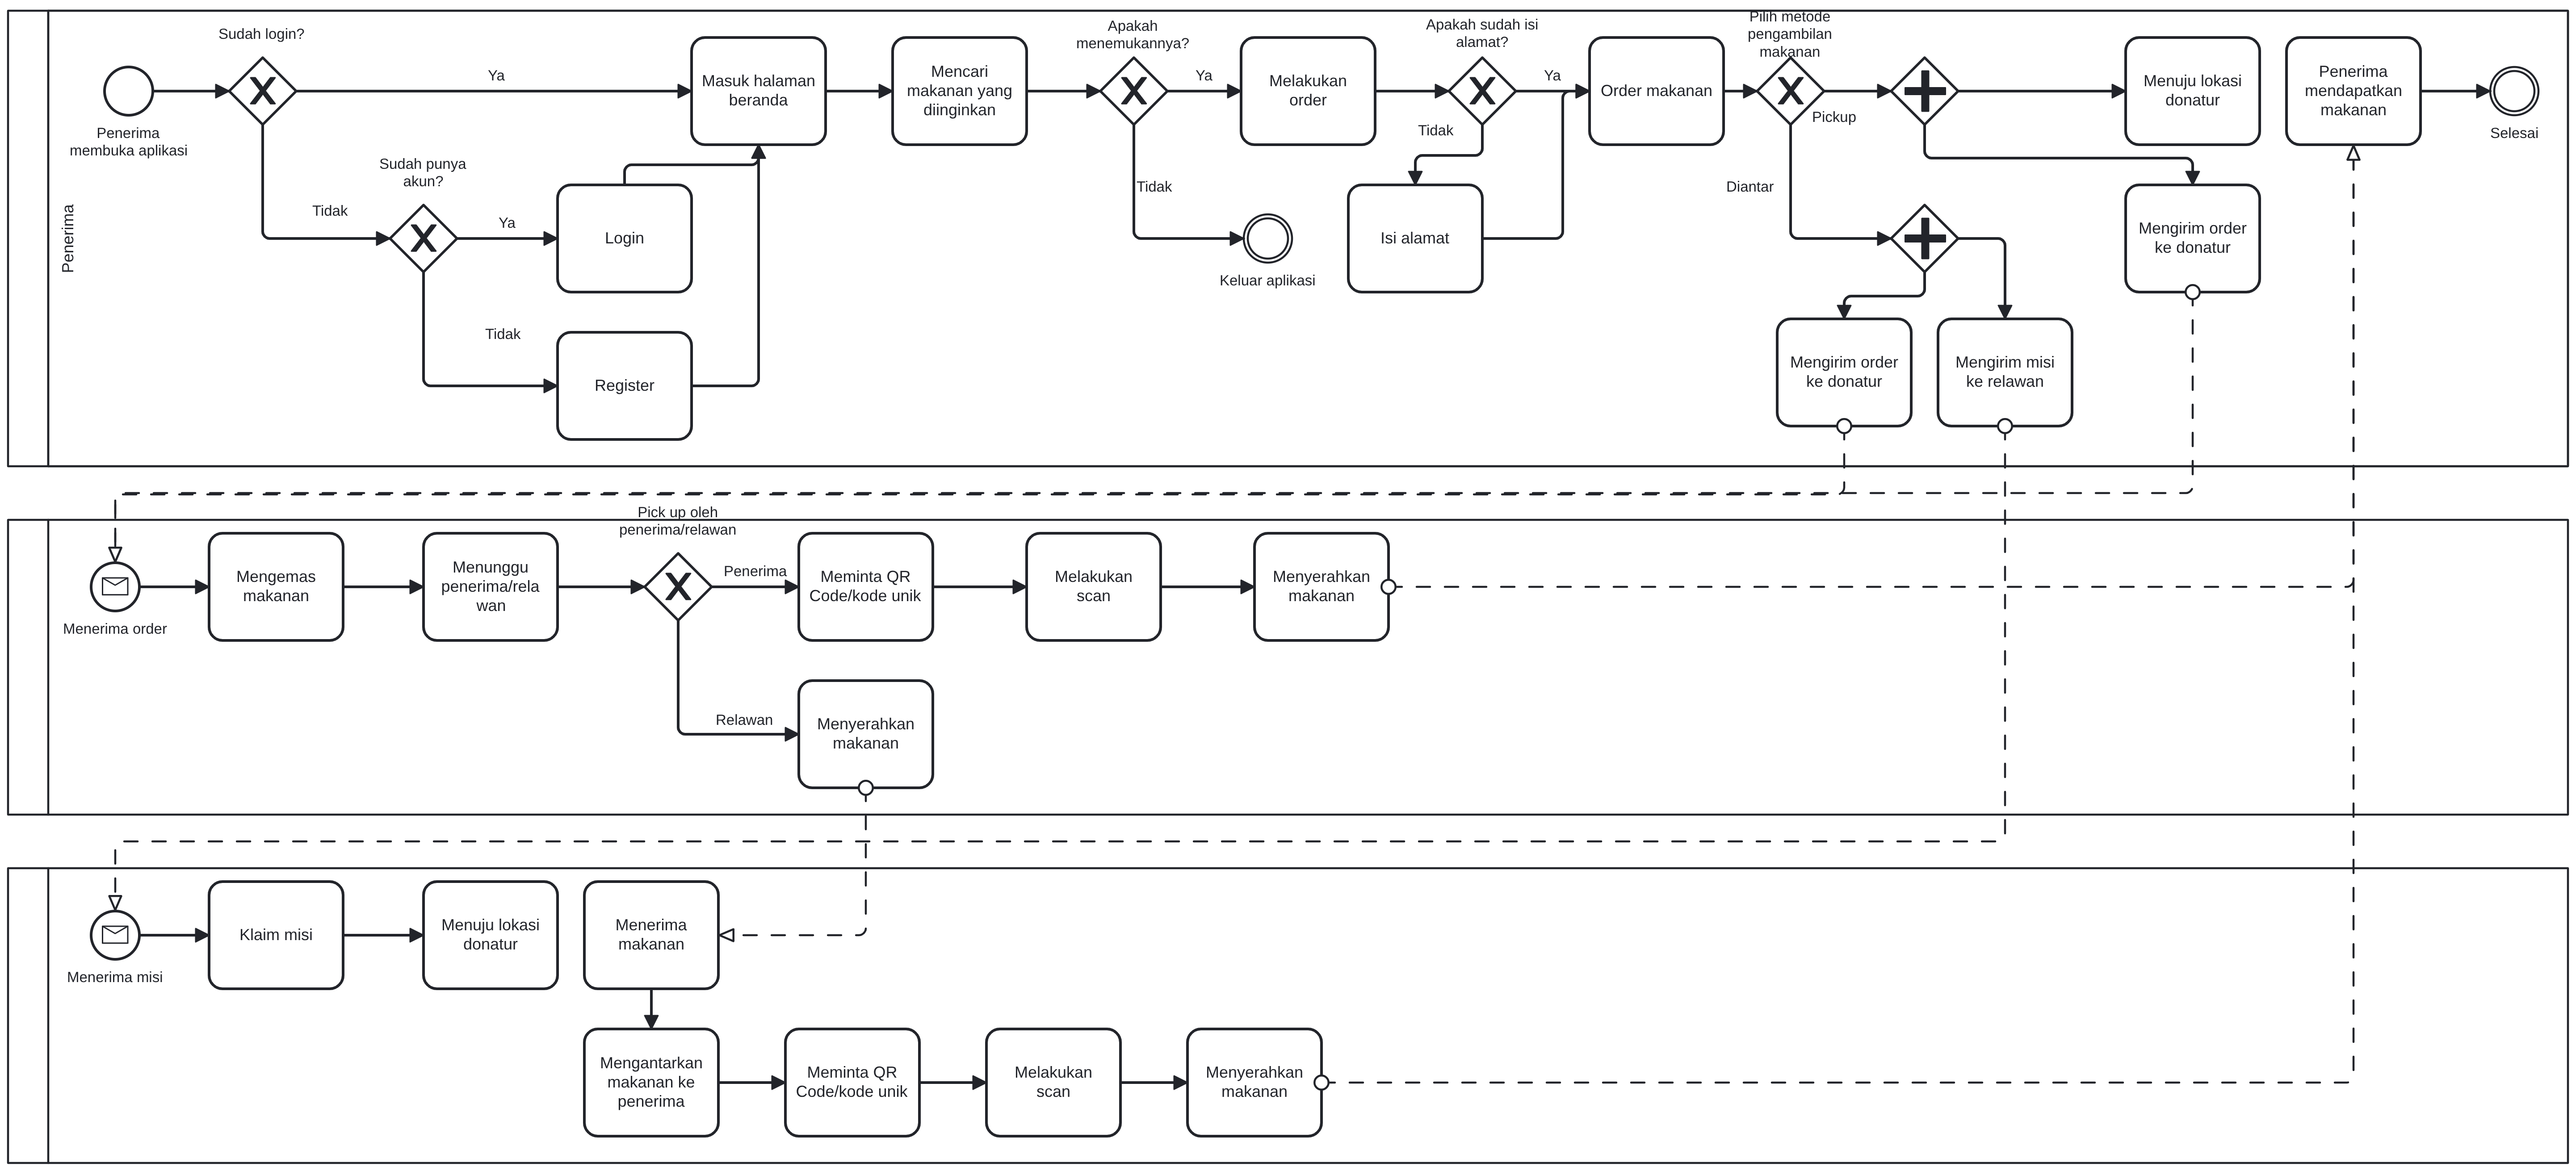
\includegraphics[width=0.9\linewidth]{image/bpmnToBe.png}
    \captionof{figure}{Proses Bisnis Sistem Usulan (BPMN To-Be)}
    \label{fig:bpmnToBe}
    \vfill
\end{landscape}

\newpage

\subsection{Pengalaman Pengguna}
Guna memastikan bahwa platform Food AI Rescue yang dikembangkan dapat menyelesaikan permasalahan secara akurat dan tepat sasaran, penelitian ini menerapkan pendekatan desain berpusat pada manusia (\textit{Human-Centered Design}). Pendekatan ini secara spesifik memetakan pengalaman dari target pengguna utama di lapangan, yakni pihak donatur, penerima donasi, dan relawan logistik, ketika mereka masih melakukan proses penyaluran surplus makanan secara manual atau konvensional (\textit{As-Is}). Hasil pemetaan permasalahan tersebut kemudian dituangkan ke dalam tiga artefak \textit{User Experience} (UX), meliputi \textit{User Persona}, \textit{Empathy Map}, dan \textit{User Journey Map}, yang dijabarkan sebagai berikut:

\begin{figure}[htbp]
    \centering
    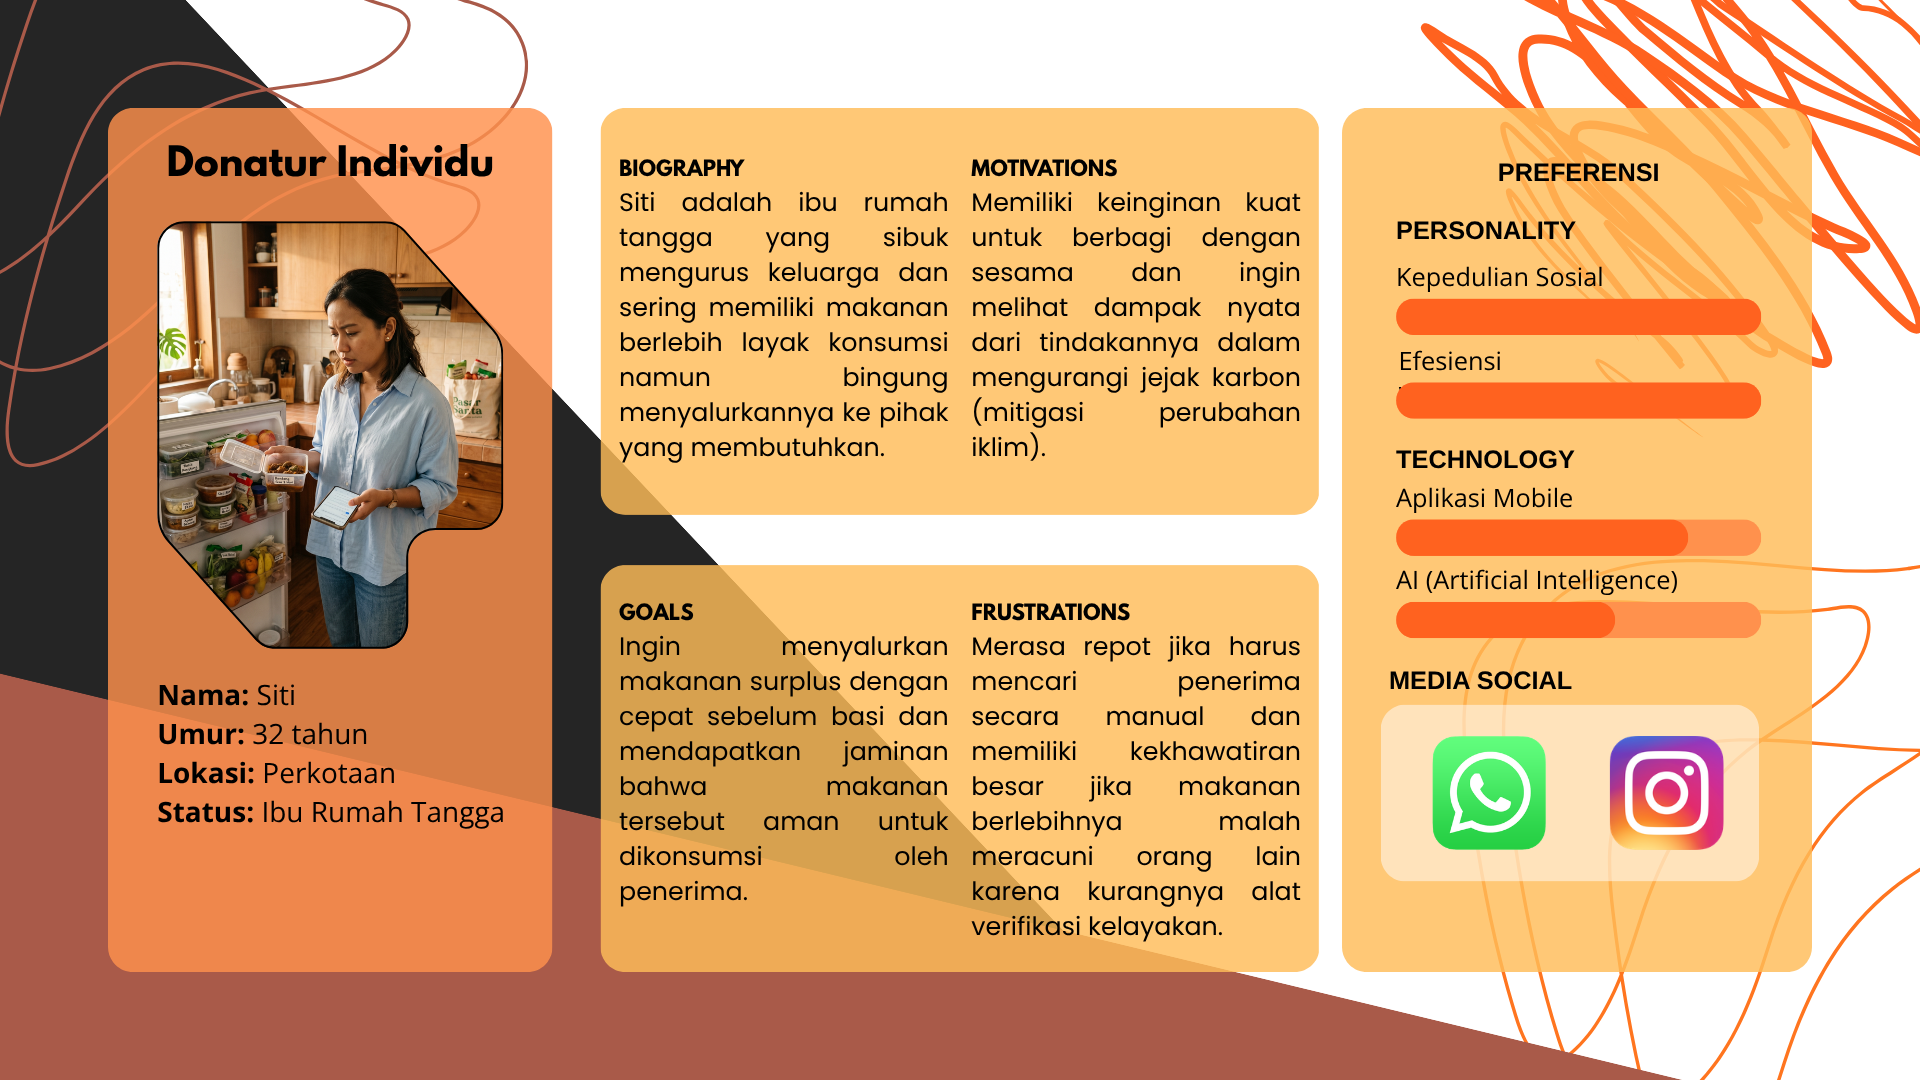
\includegraphics[width=1\textwidth]{image/bab2/User Persona/THINKS AND FEELS(1)/UP.DonaturIndividu.png}
    \caption{User Persona Individu Donor}
    \label{fig:userPersonaIndividuDonor}
\end{figure}
\begin{figure}[htbp]
    \centering
    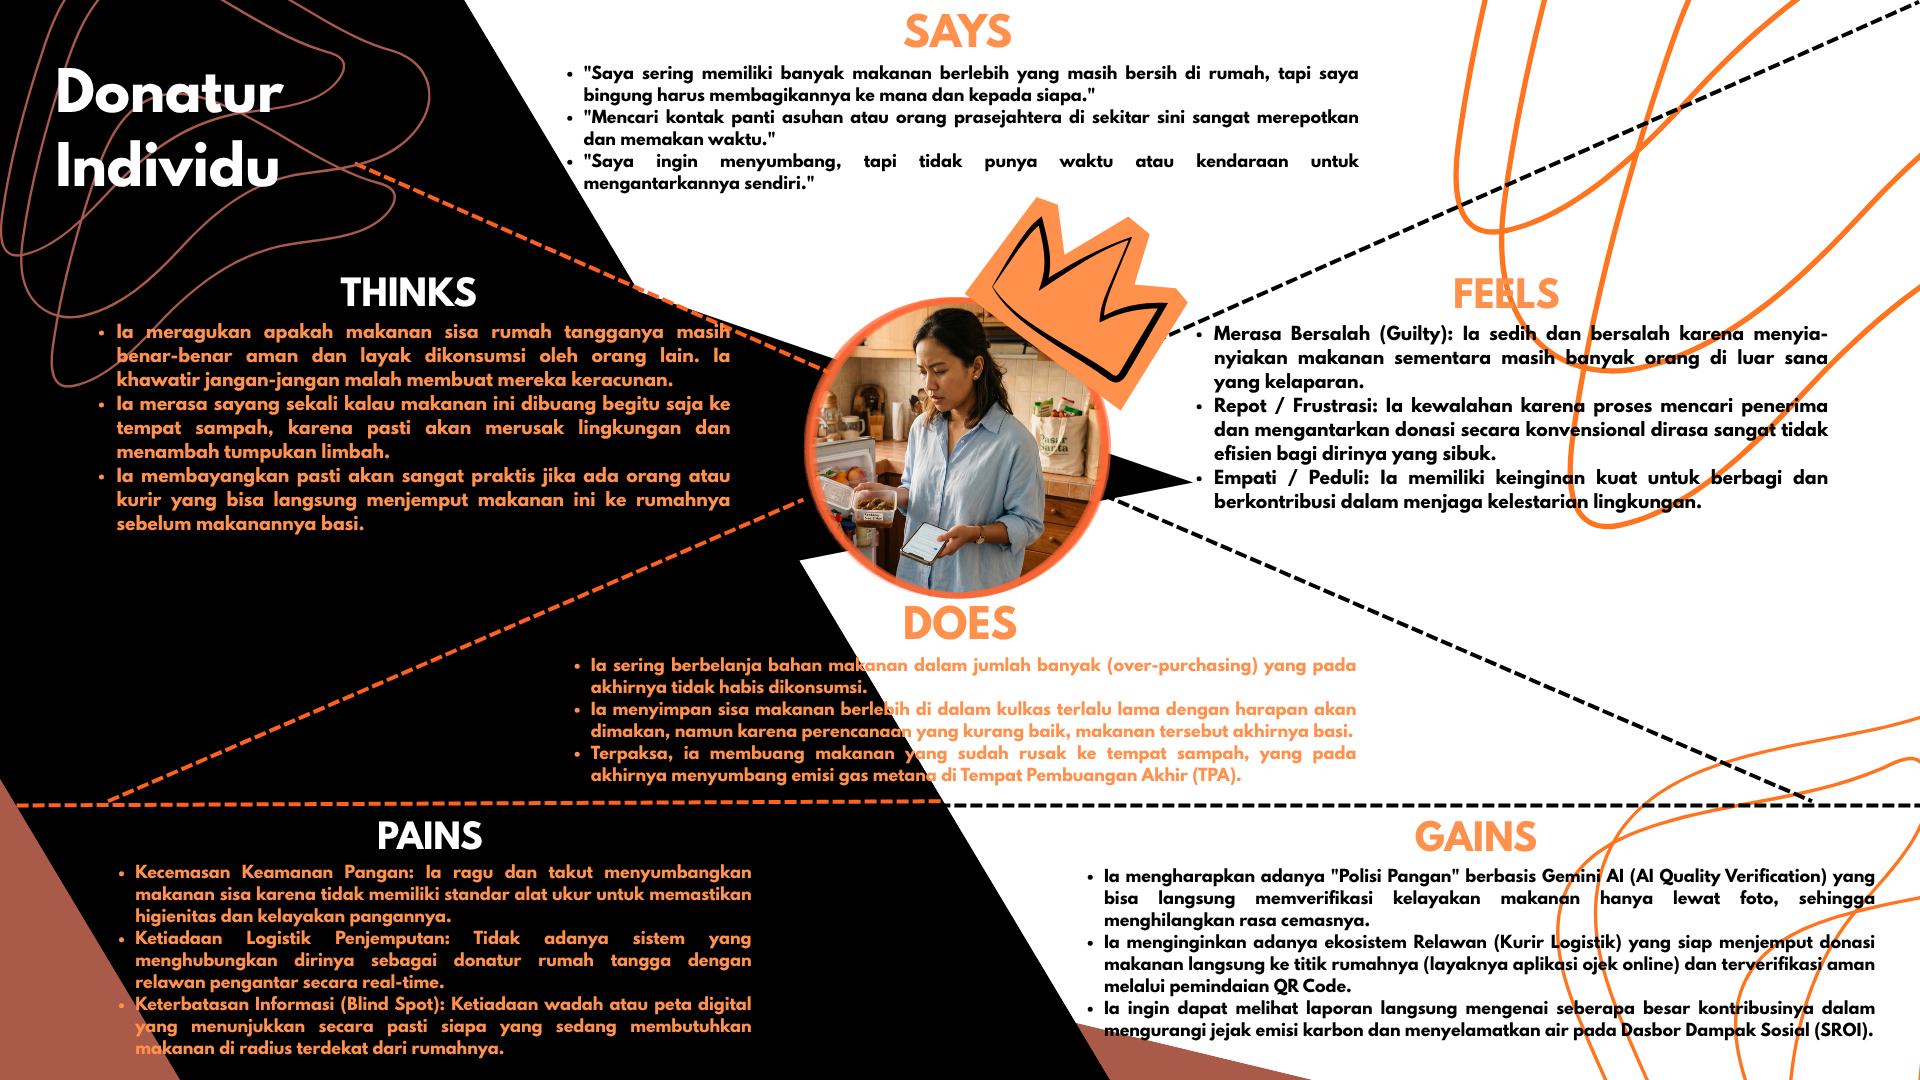
\includegraphics[width=1\textwidth]{image/bab2/segmentasi/empati_map/thinks_and_feels/donatur_individu.png}
    \caption{Empati Map Individu Donor}
    \label{fig:empatiMapIndividuDonor}
\end{figure}

\begin{figure}[htbp]
    \centering
    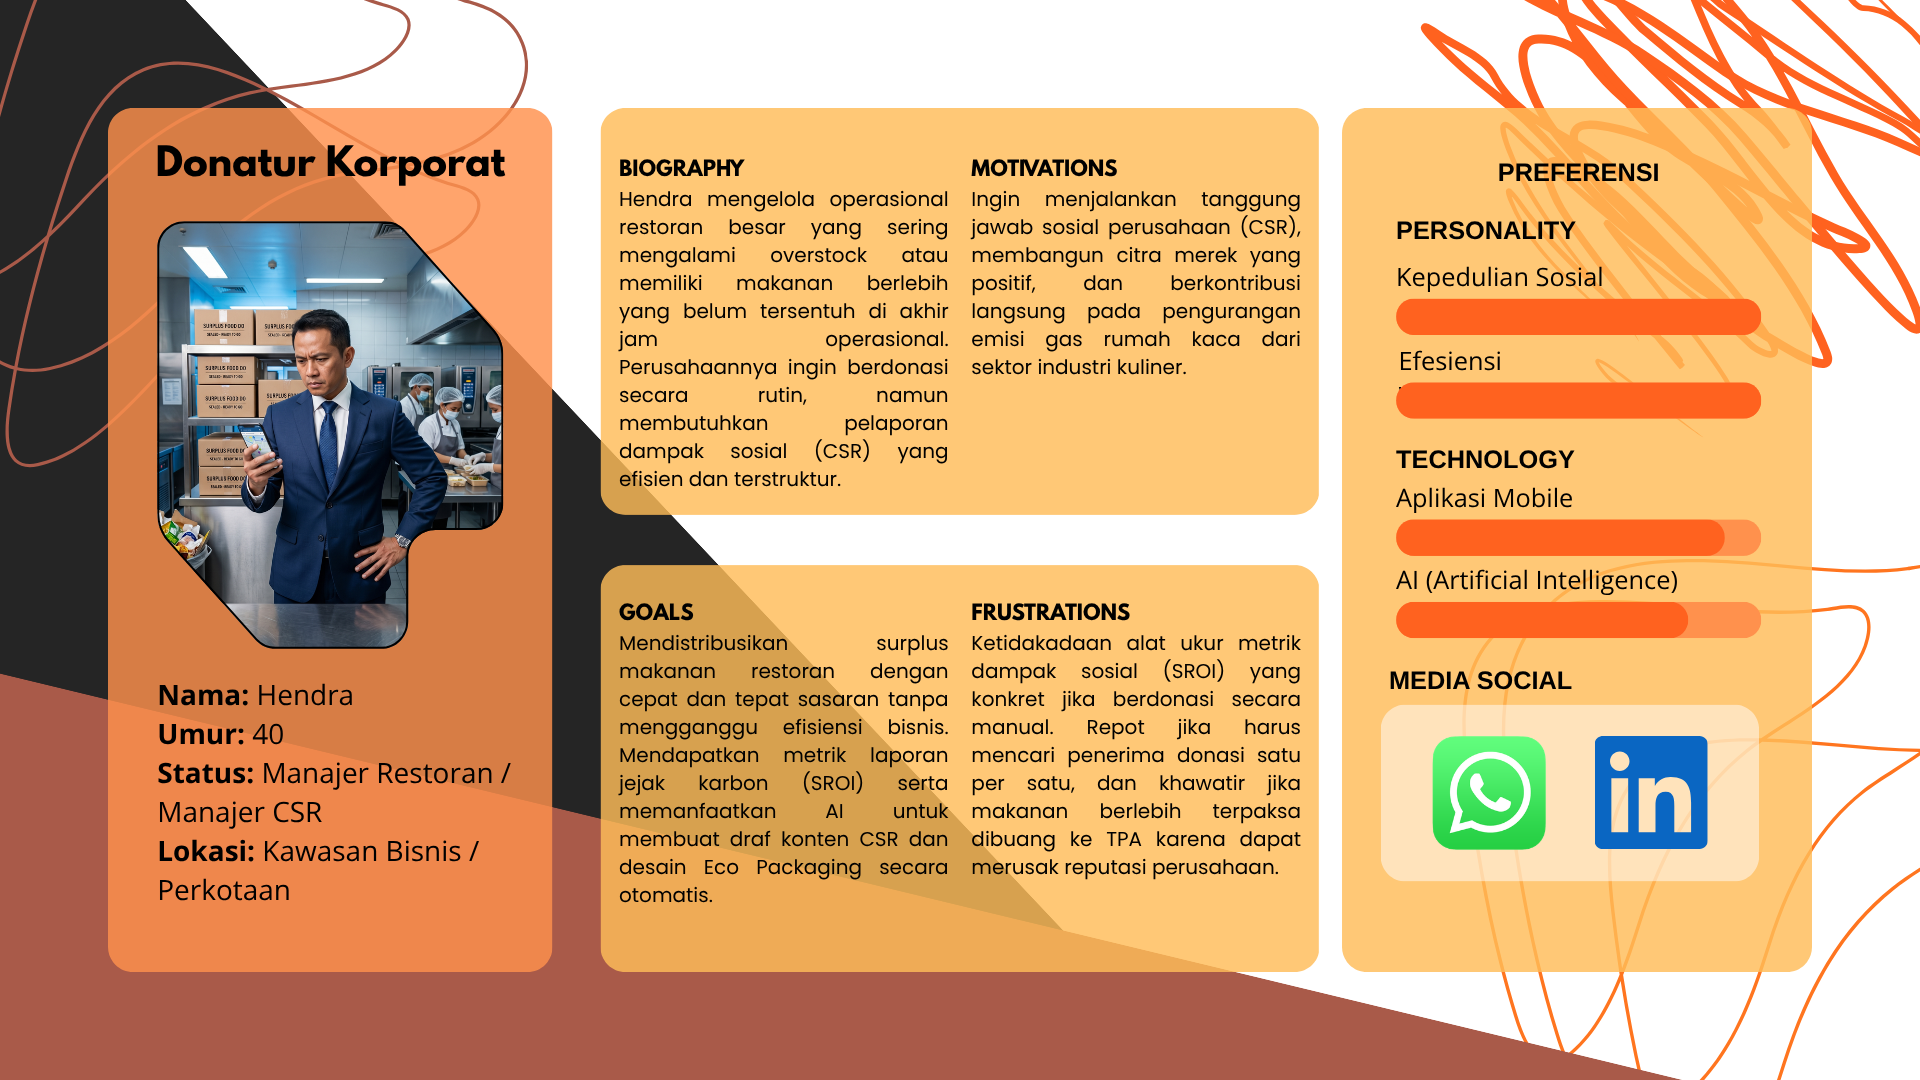
\includegraphics[width=1\textwidth]{image/bab2/User Persona/THINKS AND FEELS(1)/UP.DonaturKorporat.png}
    \caption{User Persona Korporat Donor}
    \label{fig:userPersonaKorporatDonor}
\end{figure}
\begin{figure}[htbp]
    \centering
    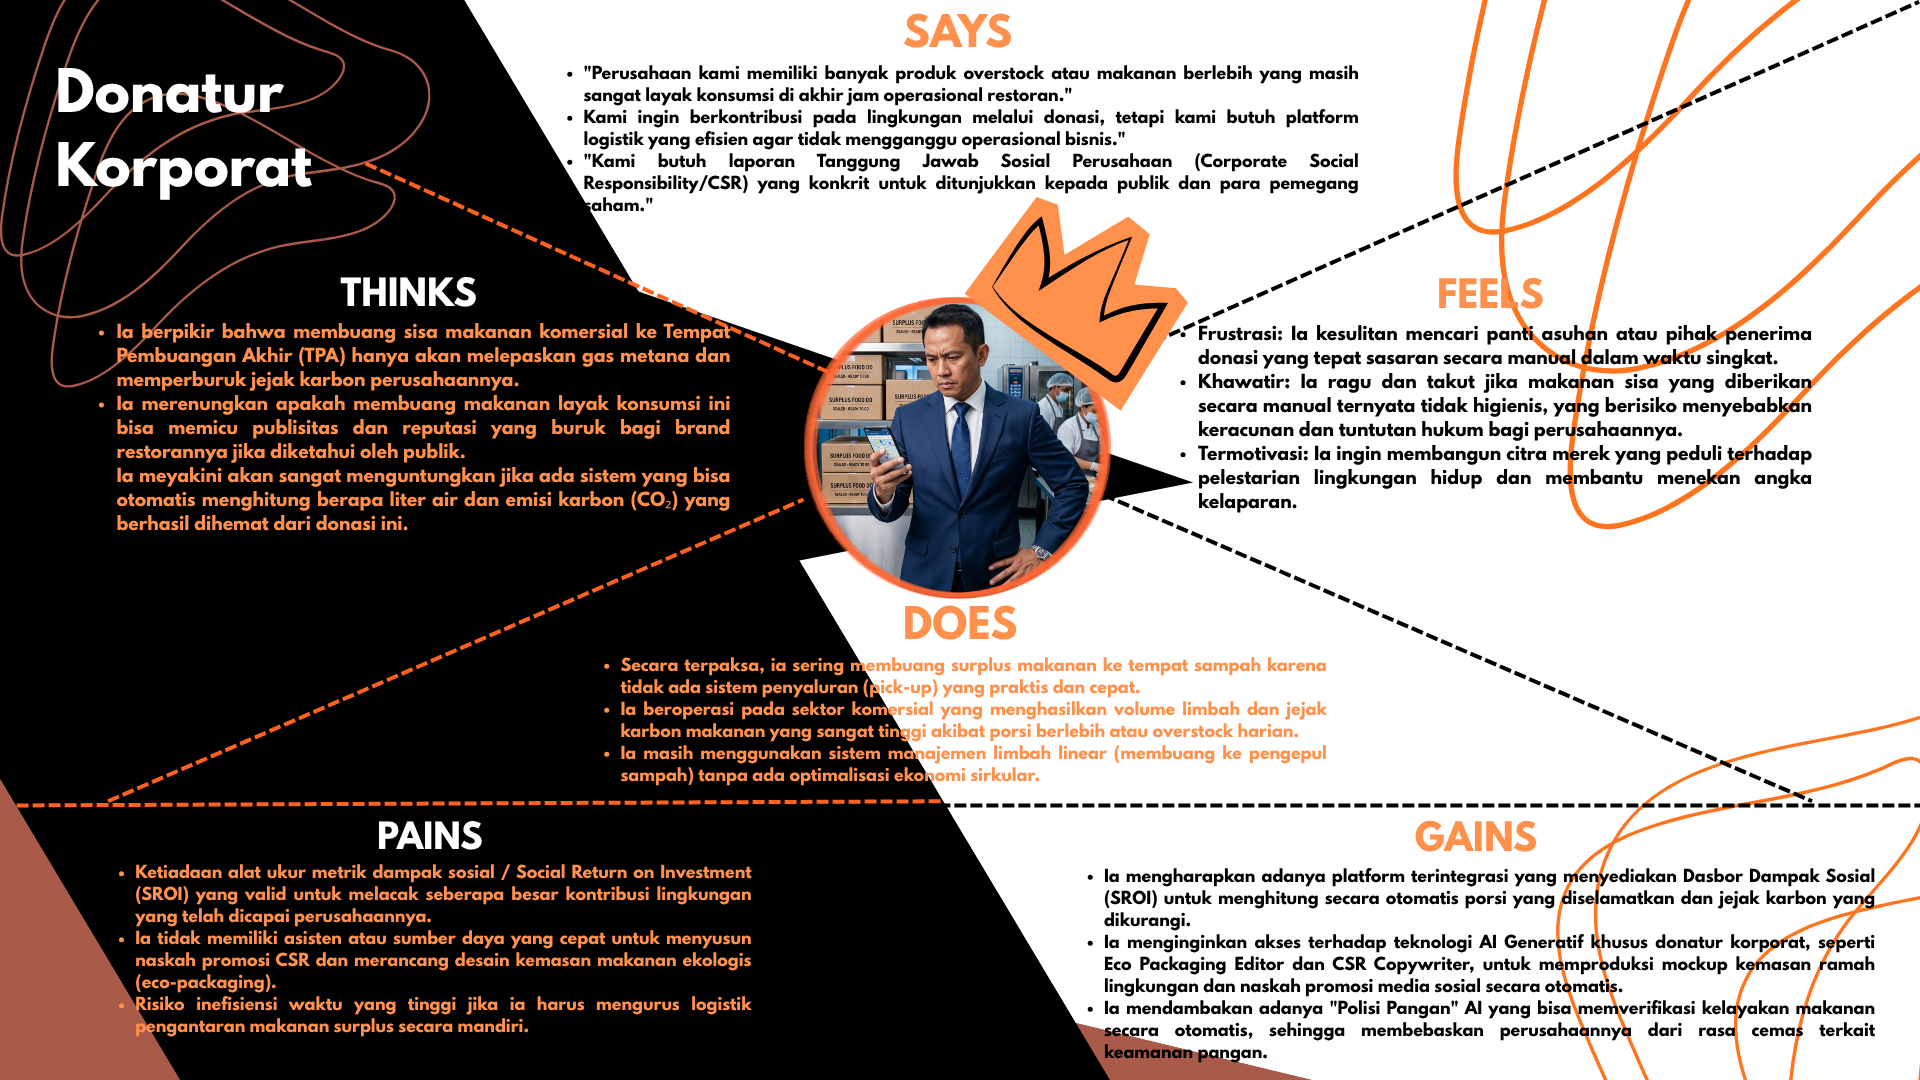
\includegraphics[width=1\textwidth]{image/bab2/segmentasi/empati_map/thinks_and_feels/donatur_korporat.png}
    \caption{Empati Map Korporat Donor}
    \label{fig:empatiMapKorporatDonor}
\end{figure}

\begin{figure}[htbp]
    \centering
    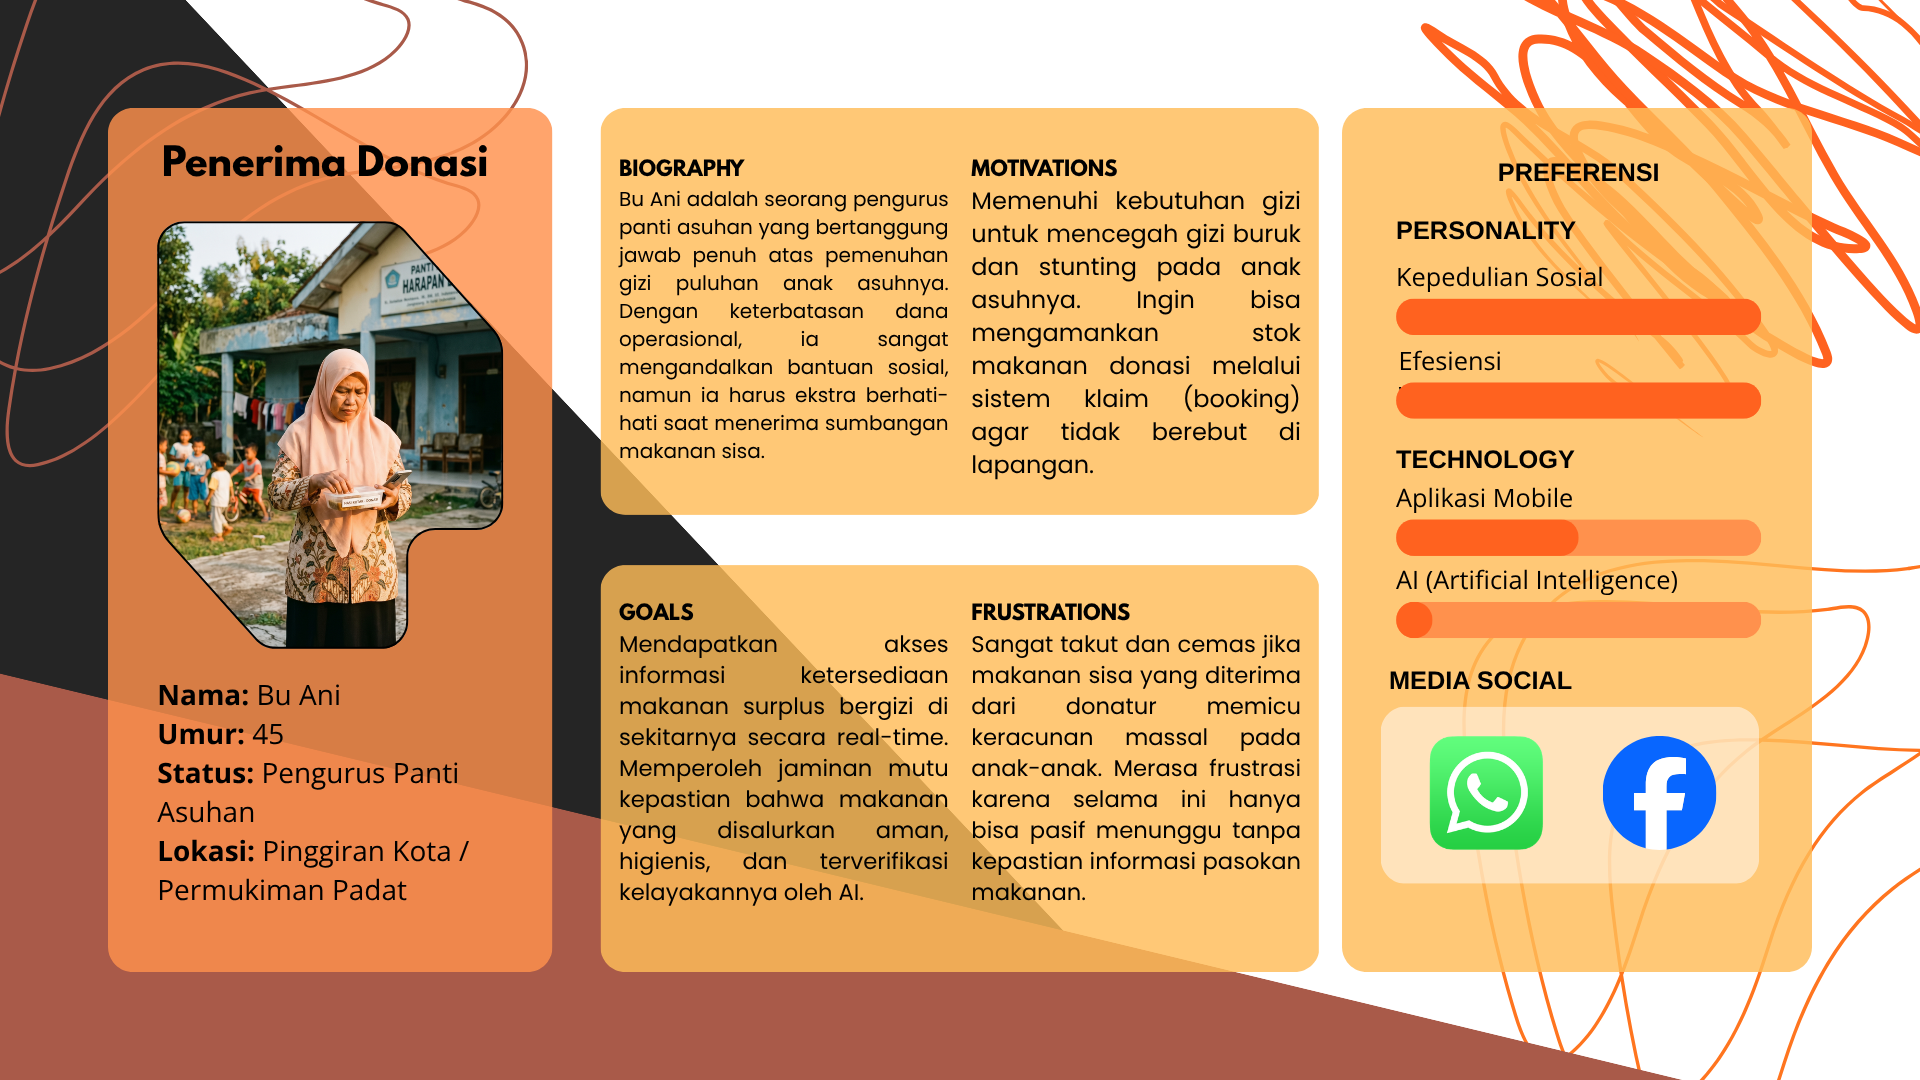
\includegraphics[width=1\textwidth]{image/bab2/User Persona/THINKS AND FEELS(1)/UP.PenerimaDonasi.png}
    \caption{User Persona Penerima}
    \label{fig:userPersonaPenerima}
\end{figure}
\begin{figure}[htbp]
    \centering
    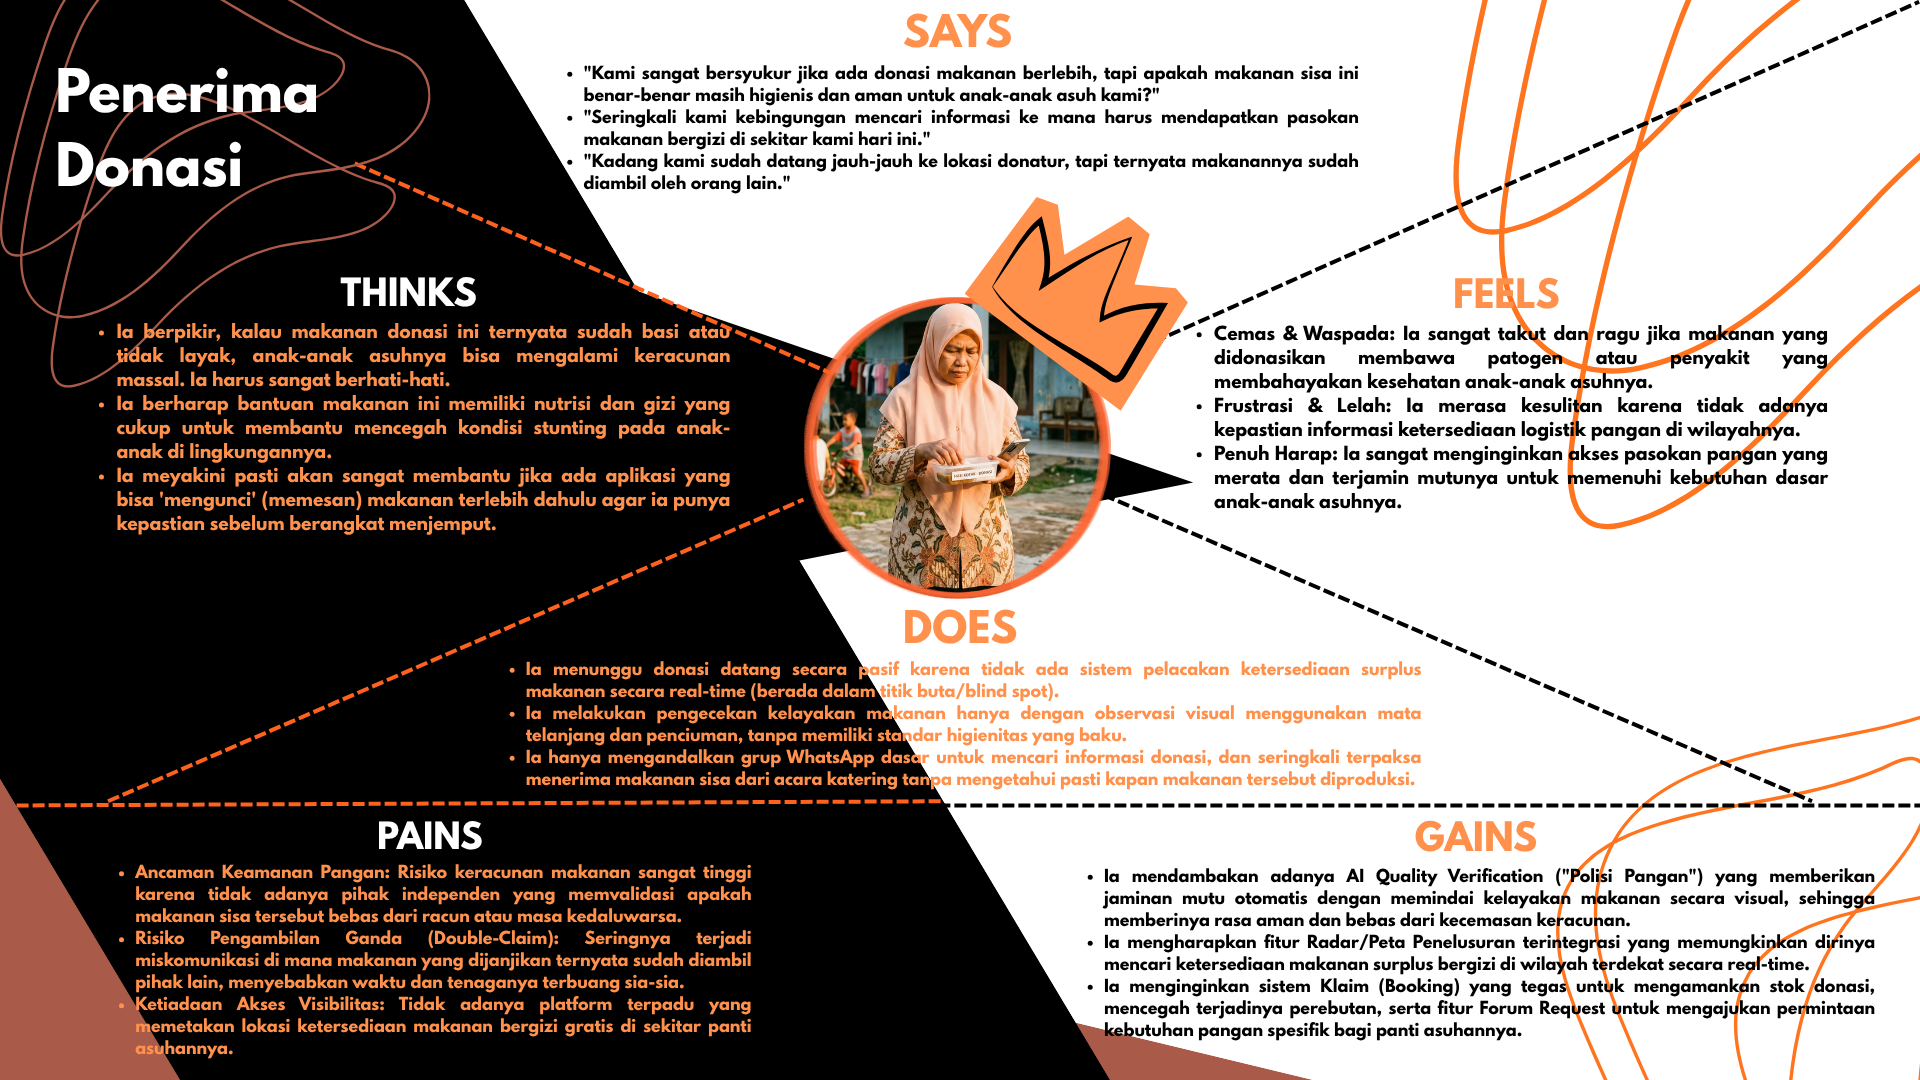
\includegraphics[width=1\textwidth]{image/bab2/segmentasi/empati_map/thinks_and_feels/penerima.png}
    \caption{Empati Map Penerima}
    \label{fig:empatiMapPenerima}
\end{figure}

\begin{figure}[htbp]
    \centering
    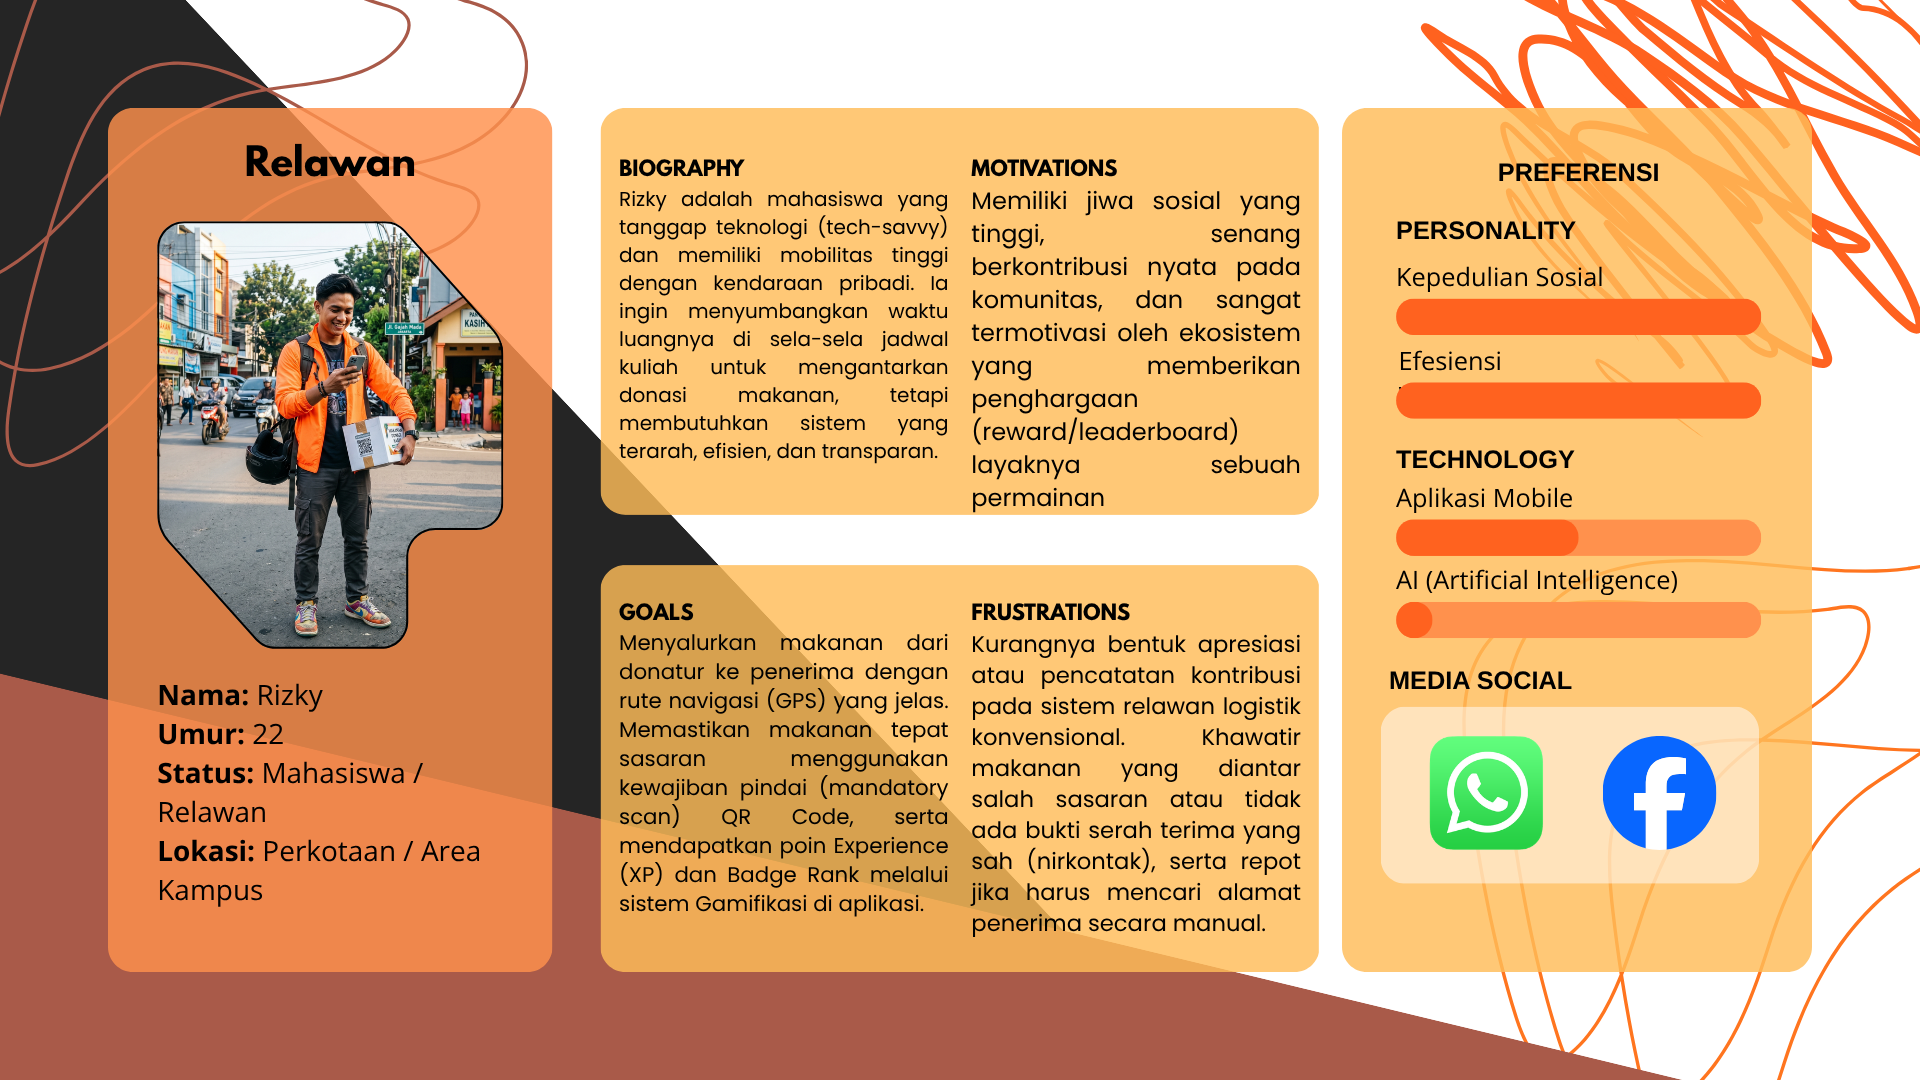
\includegraphics[width=1\textwidth]{image/bab2/User Persona/THINKS AND FEELS(1)/UP.Relawan.png}
    \caption{User Persona Relawan}
    \label{fig:userPersonaRelawan}
\end{figure}
\begin{figure}[htbp]
    \centering
    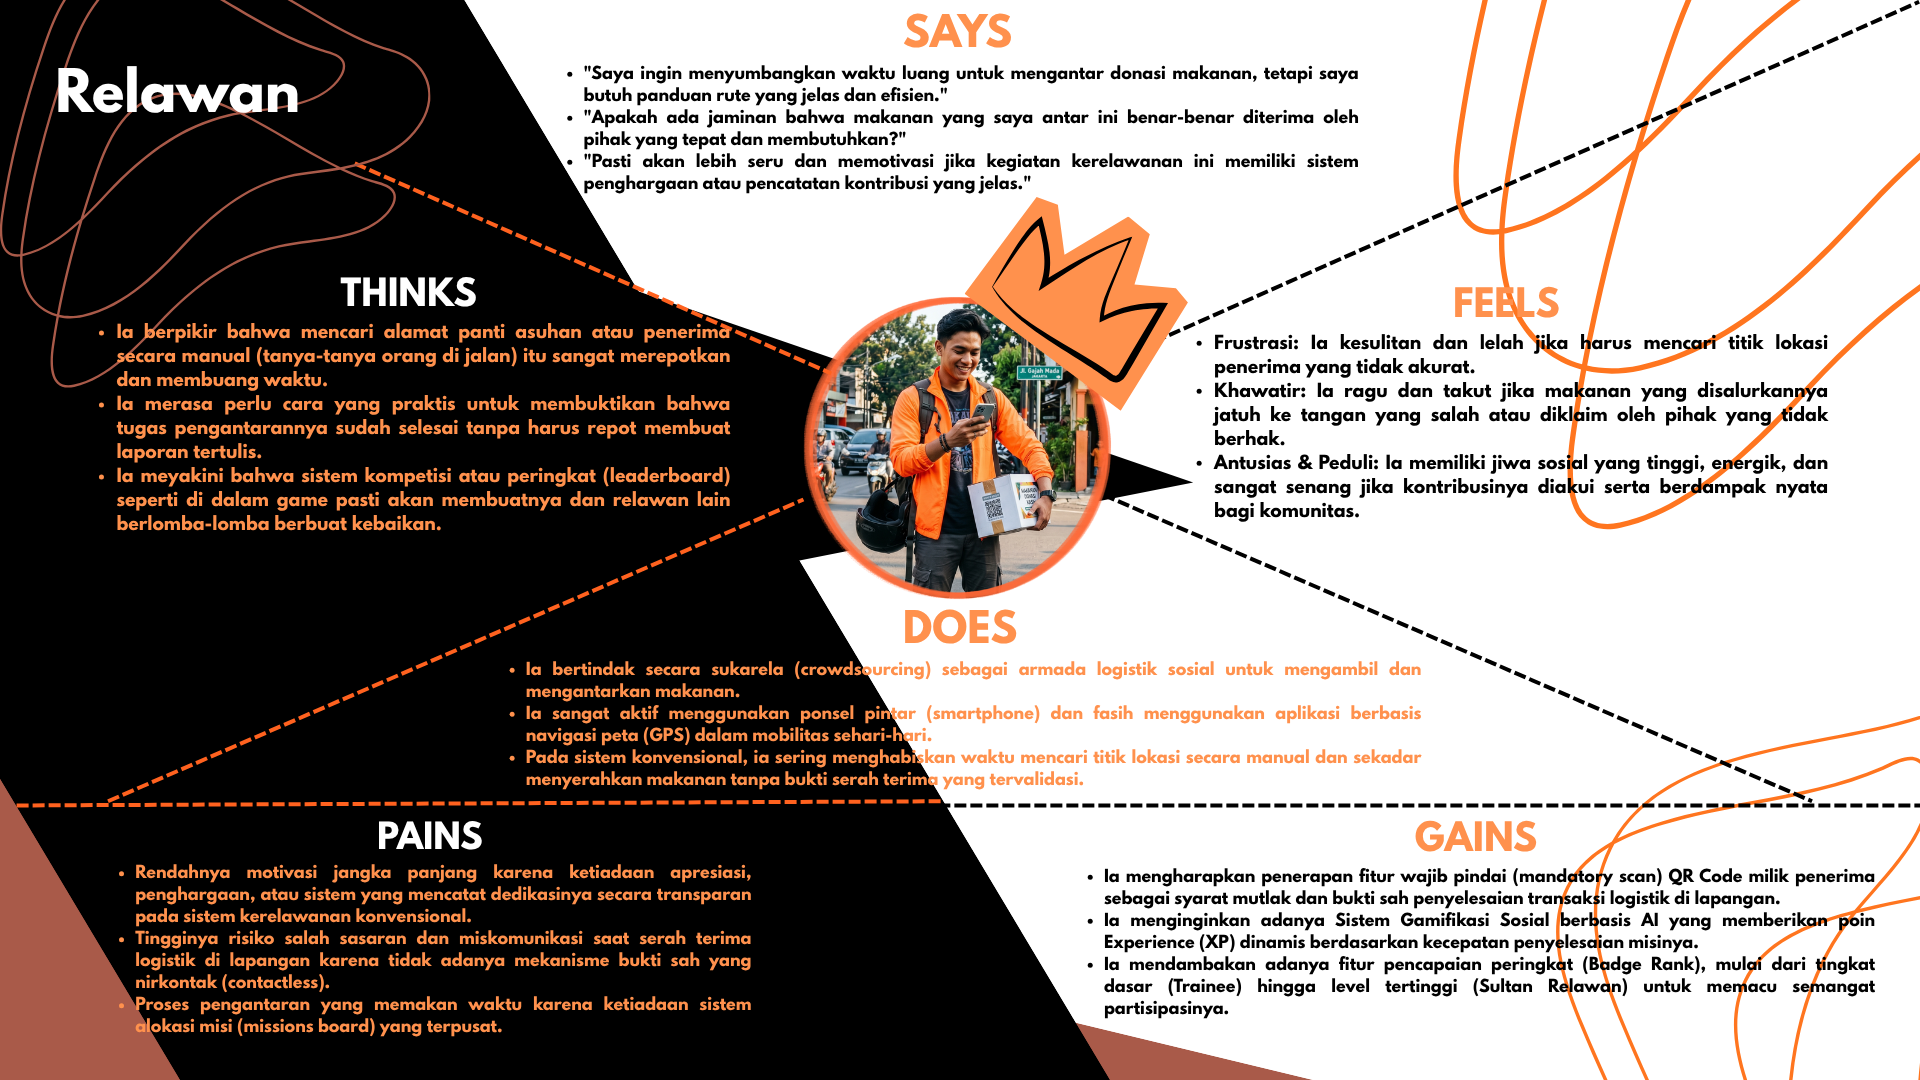
\includegraphics[width=1\textwidth]{image/bab2/segmentasi/empati_map/thinks_and_feels/relawan.png}
    \caption{Empati Map Relawan}
    \label{fig:empatiMapRelawan}
\end{figure}
\clearpage

\section{Identifikasi Aplikasi Sejenis}
\par Tahapan identifikasi aplikasi sejenis merupakan langkah analitis yang dilakukan untuk memetakan produk atau platform digital pendahulu (\textit{existing solutions}) yang memiliki kesamaan fungsional dengan sistem yang diusulkan. Tujuan utama dari observasi ini adalah untuk menemukan celah kelemahan (\textit{gap}) serta batasan operasional pada aplikasi yang telah beredar di masyarakat. Melalui analisis komparatif ini, pengembangan platform Food AI Rescue dapat difokuskan untuk merancang nilai tambah (\textit{value proposition}) yang lebih inovatif, tepat sasaran, dan relevan dalam menjembatani kebutuhan para pemangku kepentingan di ekosistem donasi pangan.

\par Dalam observasi ini, perbandingan difokuskan pada empat platform pengelola sisa makanan yang menjadi tolok ukur dalam inisiatif food rescue, yaitu:
\begin{enumerate}
    \item Surplus Indonesia: Aplikasi \textit{food rescue} komersial yang berfokus menyelamatkan makanan berlebih dari pelaku usaha (restoran, hotel, katering) dengan memfasilitasi pelanggan untuk membeli makanan yang belum habis terjual tersebut di akhir jam operasional dengan potongan harga hingga setengahnya.
    \item Garda Pangan: Organisasi \textit{food bank} di Indonesia yang berfokus pada penyelamatan surplus makanan dari industri \textit{hospitality} dan mendistribusikannya secara gratis kepada masyarakat pra-sejahtera melalui operasional jaringan relawan secara konvensional.
    \item Foodbank of Indonesia (FOI): Jaringan nirlaba nasional yang mengelola distribusi donasi dan makanan berlebih dari berbagai pihak untuk mencegah kelaparan, dengan fokus kampanye pada perbaikan gizi anak-anak balita dan kelompok rentan di berbagai wilayah.
    \item Too Good To Go: Aplikasi global pionir \textit{food rescue} (populer di Eropa dan Amerika) yang menghubungkan pelanggan dengan restoran atau toko kelontong untuk membeli ``paket kejutan'' (\textit{magic bags}) berisi makanan sisa layak konsumsi dengan harga yang sangat murah.
\end{enumerate}

\par Rincian perbandingan fitur dan kapabilitas layanan antara platform kompetitor dengan sistem Food AI Rescue yang diusulkan dapat diringkas pada tabel berikut:

\begin{table}[htbp]
    \centering
    \renewcommand{\arraystretch}{1.5}
    \caption{Perbandingan Fitur dan Kapabilitas Layanan Platform Food Rescue}
    \label{tab:perbandingan_fitur}
    \begin{tabularx}{\textwidth}{|L|C|C|C|C|C|}
        \hline
        \rowcolor{gray!10} \textbf{Fitur / Layanan Utama} & \textbf{Surplus Indonesia} & \textbf{Garda Pangan} & \textbf{Foodbank of Indonesia} & \textbf{Too Good To Go} & \textbf{Food AI Rescue (Usulan)} \\ \hline
        Penyaluran Donasi Makanan Secara Gratis & \xmark & \cmark & \cmark & \xmark & \cmark \\ \hline
        Verifikasi Kelayakan Makanan Otomatis (AI) & \xmark & \xmark & \xmark & \xmark & \cmark \\ \hline
        Sistem Penjemputan oleh Relawan Tergamifikasi & \xmark & \xmark & \xmark & \xmark & \cmark \\ \hline
        Validasi Serah Terima Nirkontak (QR Code) & \xmark & \xmark & \xmark & \xmark & \cmark \\ \hline
        Dasbor Kalkulasi Dampak Sosial (SROI) \textit{Real-Time} & \xmark & \xmark & \xmark & \xmark & \cmark \\ \hline
        Fitur AI Generatif untuk Kampanye CSR Korporat & \xmark & \xmark & \xmark & \xmark & \cmark \\ \hline
    \end{tabularx}
\end{table}

\newpage

\par Berdasarkan Tabel \ref{tab:perbandingan_fitur} di atas, dapat diidentifikasi beberapa celah (\textit{gap}) fungsionalitas yang menjadi landasan utama pengembangan Food AI Rescue. Platform komersial seperti Surplus Indonesia dan Too Good To Go sangat unggul dalam menyelamatkan sisa makanan dengan cepat, namun berfokus pada model transaksi jual-beli diskon, sehingga belum sepenuhnya menyasar masyarakat prasejahtera yang membutuhkan donasi secara cuma-cuma. Sementara itu, inisiatif sosial seperti Garda Pangan dan Foodbank of Indonesia memiliki rekam jejak penyaluran donasi gratis yang sangat baik, namun operasional logistiknya masih bersifat konvensional dan sangat bergantung pada verifikasi kelayakan makanan secara manual oleh manusia.

\par Lebih jauh lagi, keempat platform pembanding tersebut umumnya belum mengadopsi teknologi mutakhir seperti Kecerdasan Buatan (AI). Belum tersedia fitur otomatisasi yang mampu memverifikasi standar keamanan dan higienitas makanan secara visual (\textit{Computer Vision}), serta belum ada pelacakan metrik dampak lingkungan yang komprehensif. Platform pendahulu juga belum menyediakan dukungan fitur khusus yang memfasilitasi kebutuhan pelaporan donatur korporat dalam satu pusat kendali (\textit{dashboard}).

\par Oleh karena itu, usulan pengembangan Food AI Rescue hadir dengan posisi tawar (\textit{value proposition}) yang unik. Food AI Rescue menggabungkan penyaluran donasi pangan gratis, validasi keamanan berbasis AI (``Polisi Pangan''), dan operasional penjemputan logistik berbasis gamifikasi relawan ke dalam satu aplikasi yang ramah pengguna. Keberadaan Dasbor Dampak Sosial (SROI) \textit{real-time} serta pemisahan hak akses berbasis peran (\textit{Role-Based Access Control}) antara donatur, penerima, relawan, dan admin menjadikan platform ini tidak hanya sebagai alat penyalur bantuan teknis, tetapi juga sebagai ekosistem manajemen komunitas ketahanan pangan cerdas yang aman, transparan, dan terpadu.

\section{Analisis Kebutuhan Sistem}
Analisis persyaratan sistem merupakan langkah esensial dalam mentransformasikan kendala operasional pada sistem manual (As-Is) serta titik keluhan (pain points) para aktor lapangan ke dalam spesifikasi teknis yang komprehensif bagi platform Food AI Rescue. Tahapan analisis ini diklasifikasikan ke dalam tiga segmen utama, yakni pendefinisian tingkat hak akses pengguna (meliputi Donatur, Penerima, Relawan, Admin, dan SuperAdmin), pemetaan kebutuhan fungsional cerdas aplikasi, serta spesifikasi infrastruktur teknologi pendukung di sisi backend.

\subsection{Analisis Grup Akses}
\par Berdasarkan deskripsi pengguna dan pemetaan empati dari hasil rancangan \textit{User Persona}, terlihat jelas bahwa pengguna pada ekosistem aplikasi ini memiliki latar belakang literasi teknologi serta tanggung jawab operasional yang sangat bervariasi. Untuk mencegah pengguna awam kebingungan saat menavigasi fitur aplikasi, serta guna melindungi stabilitas infrastruktur sistem, seperti basis data dan konfigurasi Kecerdasan Buatan (AI), dari risiko penyalahgunaan atau kesalahan pengaturan (\textit{human error}), maka platform Food AI Rescue dirancang menggunakan arsitektur keamanan \textit{Role-Based Access Control} (RBAC).

\par Sistem ini membagi pengguna ke dalam 6 (enam) grup akses (\textit{role}) utama dengan pembatasan wewenang, fungsionalitas, dan pemanfaatan Kecerdasan Buatan (AI) yang sangat spesifik, yaitu:

\begin{enumerate}
    \item \textbf{Donatur Individu}
    \begin{itemize}
        \item \textbf{Peranan}: Pengguna dari kalangan masyarakat perorangan atau pelaku usaha skala mikro yang memiliki kelebihan produksi makanan layak konsumsi dalam jumlah kecil (skala rumah tangga).
        \item \textbf{Hak Akses}: Memiliki wewenang operasional untuk mengunggah data makanan surplus, memperbarui status ketersediaan (\textit{inventory}), dan melakukan serah terima donasi dengan wajib memindai Kode QR milik penerima sebagai bukti sah. Donatur individu juga berhak memantau Dasbor Dampak Sosial (SROI) secara langsung, serta menggunakan hak akses AI \textit{Quality Verification} (Polisi Pangan) untuk memvalidasi kelayakan makanan dan mendapatkan rekomendasi resep masakan.
    \end{itemize}

    \item \textbf{Donatur Kelompok/Korporat (Mitra Penyedia)}
    \begin{itemize}
        \item \textbf{Peranan}: Pengguna dari entitas bisnis skala besar, khususnya di sektor HORECA (Hotel, Restoran, dan Kafe), atau usaha katering berskala komersial yang menyumbangkan surplus makanan secara masif.
        \item \textbf{Hak Akses}: Memiliki wewenang manajemen distribusi dan pemantauan SROI yang sama dengan Donatur Individu. Sebagai nilai tambah untuk kebutuhan \textit{Corporate Social Responsibility} (CSR), peran ini dibekali hak akses AI Generatif eksklusif yang meliputi fitur \textit{Eco Packaging Editor} untuk merancang desain kemasan ramah lingkungan, dan fitur \textit{CSR Copywriter} untuk otomatisasi pembuatan naskah kampanye sosial.
    \end{itemize}

    \item \textbf{Penerima (Mitra Penerima)}
    \begin{itemize}
        \item \textbf{Peranan}: Kelompok masyarakat di kawasan rentan pangan, fasilitas sosial (seperti panti asuhan), dewan kemakmuran masjid (DKM), atau warga prasejahtera yang bertindak sebagai sasaran distribusi donasi.
        \item \textbf{Hak Akses}: Memiliki wewenang untuk mengakses radar peta (\textit{Map Dashboard}), mencari menu makanan terdekat, melakukan klaim (\textit{booking}) guna mencegah pengambilan ganda (\textit{double-claim}), dan menyajikan Kode QR miliknya untuk dipindai saat makanan tiba. Grup ini juga diberi hak untuk memberikan ulasan (\textit{feedback}), mengajukan permintaan spesifik via \textit{Forum Request}, serta menggunakan AI \textit{Quality Verification} untuk mengecek makanan sebelum dikonsumsi.
    \end{itemize}

    \item \textbf{Relawan (Kurir)}
    \begin{itemize}
        \item \textbf{Peranan}: Pengguna dari kalangan pemuda lokal atau masyarakat umum yang berpartisipasi secara sukarela (\textit{crowdsourcing}) sebagai armada penggerak logistik sosial penjemputan makanan.
        \item \textbf{Hak Akses}: Berwenang untuk mengakses daftar papan misi pengantaran, melakukan penjemputan makanan dari lokasi donatur, dan mengantarkannya ke titik lokasi penerima. Relawan memegang otoritas validasi lapangan dengan hak akses wajib pindai (\textit{mandatory scan}) Kode QR nirkontak sebagai syarat mutlak penyelesaian transaksi, yang secara otomatis terintegrasi dengan sistem poin gamifikasi (\textit{Leaderboard Ranking}).
    \end{itemize}

    \item \textbf{Admin Pengelola}
    \begin{itemize}
        \item \textbf{Peranan}: Tim manajerial dan pengawas operasional harian yang bertugas mengelola platform secara administratif di tingkat komunitas.
        \item \textbf{Hak Akses}: Memiliki wewenang administratif untuk memverifikasi pendaftaran akun baru, memblokir akun yang melakukan penyalahgunaan, menangani keluhan pengguna (\textit{support request}), serta memantau Dasbor Statistik (SROI) dan peta panas (\textit{heatmap}) sebaran donasi. Dari sisi kecerdasan buatan, Admin dibekali hak modifikasi panel \textit{Prompt Engineering} untuk menyesuaikan parameter instruksi deteksi AI secara \textit{real-time} tanpa perlu mengubah kode sumber aplikasi.
    \end{itemize}

    \item \textbf{Super Admin}
    \begin{itemize}
        \item \textbf{Peranan}: Pengguna dengan tingkat literasi teknologi tertinggi yang bertindak sebagai pengembang sistem (Tim IT / \textit{Programmer}) dan pemegang kedaulatan mutlak platform eksekutif.
        \item \textbf{Hak Akses}: Memiliki wewenang manajerial penuh terhadap operasional sistem di sisi peladen (\textit{backend}). Akses difokuskan pada manajemen tingkat makro seperti pemeliharaan server (\textit{Maintenance Mode}), perbaikan \textit{bug}, menjaga stabilitas basis data, mengelola pendaftaran akun Admin biasa, serta mengawasi hak prerogatif akses komputasi AI dan memonitor jejak \textit{log} sistem secara keseluruhan.
    \end{itemize}
\end{enumerate}

\subsection{Analisis Kebutuhan Fungsional}
Analisis kebutuhan fungsional menguraikan spesifikasi kapabilitas yang wajib dimiliki oleh sistem guna menjawab permasalahan pengguna di lapangan. Merujuk pada hasil observasi alur distribusi manual (As-Is) serta ekstraksi titik keluhan (\textit{pain points}) dari \textit{Empathy Map} dan \textit{User Journey Map}, platform yang dirancang harus mampu menghadirkan solusi berupa otomatisasi verifikasi kelayakan pangan berbasis Kecerdasan Buatan (AI), pencocokan donasi secara \textit{real-time}, serta rekapitulasi pelaporan dampak lingkungan (SROI) secara digital. Oleh karena itu, fungsionalitas yang akan diimplementasikan pada ekosistem Food AI Rescue diklasifikasikan ke dalam tujuh modul utama berikut:

\begin{enumerate}
    \item \textbf{Kebutuhan Modul Autentikasi dan Manajemen Akun}
    \begin{itemize}
        \item Sistem harus mampu memfasilitasi proses pendaftaran (\textit{register}) dan masuk (\textit{login}) yang keamanannya terenkripsi menggunakan algoritma sandi berlapis \textit{bcrypt}.
        \item Sistem harus memiliki pendeteksi perutean berbasis peran (\textit{Role-Based Router}) untuk mengarahkan pengguna secara spesifik ke antarmuka 6 (enam) grup akses yang berbeda (Donatur Individu, Donatur Korporat, Penerima, Relawan, Admin, dan SuperAdmin).
        \item Sistem harus menyediakan fitur manajemen profil pengguna, yang mencakup utilitas pemotongan gambar (\textit{crop image}) saat pengguna mengunggah foto \textit{avatar}.
    \end{itemize}

    \item \textbf{Kebutuhan Modul Manajemen Donasi dan Inventori (Gudang Pangan)}
    \begin{itemize}
        \item Sistem harus memfasilitasi pihak Donatur untuk membuat daftar donasi makanan baru beserta detail parameter minimum dan maksimum porsi yang tersedia.
        \item Sistem harus dilengkapi dengan manajemen inventori otomatis yang mampu menyembunyikan status tayangan donasi dari publik apabila batas waktu konsumsi (kedaluwarsa) telah terlewati.
        \item Sistem harus memfasilitasi donatur untuk melakukan validasi serah terima melalui fitur pemindaian Kode QR penerima secara nirkontak saat proses penyerahan berlangsung.
    \end{itemize}

    \item \textbf{Kebutuhan Modul Integrasi Kecerdasan Buatan (AI)}
    \begin{itemize}
        \item Sistem wajib terintegrasi dengan layanan \textit{Google Gemini Vision API} sebagai fitur ``Polisi Pangan'' untuk menjalankan verifikasi otomatis secara \textit{real-time}. AI harus mampu mendeteksi wujud makanan, menilai kelayakan konsumsi, higienitas visual, serta mengevaluasi kehalalan sebelum donasi diterbitkan.
        \item Sistem harus memfasilitasi fungsi bagi pengguna untuk memindai bahan sisa makanan guna mendapatkan rekomendasi resep masakan cerdas dari AI.
        \item Khusus bagi grup Donatur Korporat (HORECA), sistem harus menyediakan fitur AI Generatif eksklusif berupa \textit{Eco Packaging Editor} (didukung oleh Pollinations.ai) untuk merancang prototipe kemasan ramah lingkungan, serta asisten \textit{CSR Copywriter} untuk otomatisasi pembuatan naskah kampanye sosial.
    \end{itemize}

    \item \textbf{Kebutuhan Modul Eksplorasi dan Klaim (Radar Penerima)}
    \begin{itemize}
        \item Sistem harus menyediakan \textit{Map Dashboard} interaktif (memanfaatkan pustaka geolokasi \textit{Leaflet}) yang memungkinkan Mitra Penerima untuk melacak titik ketersediaan donasi pangan di sekitarnya.
        \item Sistem harus memungkinkan Penerima melakukan klaim (\textit{booking/checkout}) pesanan makanan untuk mencegah terjadinya insiden klaim ganda (\textit{double-claim}) oleh pihak lain pada stok yang sama.
        \item Sistem harus menyediakan \textit{Forum Request} yang memungkinkan Penerima untuk memublikasikan kebutuhan spesifik panti/fasilitas sosial mereka.
    \end{itemize}

    \item \textbf{Kebutuhan Modul Operasional Logistik dan Gamifikasi (Relawan)}
    \begin{itemize}
        \item Sistem harus menyediakan Papan Misi Penugasan (\textit{Missions Board}) yang merincikan titik penjemputan donatur dan titik serah terima akhir bagi armada Relawan.
        \item Sistem mewajibkan alur pemindaian silang (\textit{mandatory scan}) Kode QR menggunakan kamera aplikasi sebagai prasyarat mutlak verifikasi validitas penyelesaian distribusi logistik.
        \item Sistem harus dilengkapi mesin algoritma Gamifikasi (\textit{Leaderboard Ranking Engine}) yang secara otomatis memproses ketepatan waktu misi menjadi poin pengalaman (XP), lalu mengonversinya menjadi kasta peringkat atau medali sosial.
    \end{itemize}

    \item \textbf{Kebutuhan Modul Pelacakan Dampak Sosial (SROI)}
    \begin{itemize}
        \item Sistem harus memiliki Dasbor \textit{Sustainability Impact} terpadu yang merekapitulasi rekam jejak aktivitas donasi pengguna.
        \item Sistem harus memiliki kalkulator lingkungan yang mampu mengonversi kuantitas porsi makanan yang terselamatkan menjadi data analitik estimasi angka pengurangan emisi jejak karbon (kg CO$_2$) dan pelestarian air (liter).
    \end{itemize}

    \item \textbf{Kebutuhan Modul Konfigurasi Pusat (Admin dan SuperAdmin)}
    \begin{itemize}
        \item Sistem harus menyediakan \textit{Control Panel} operasional bagi Admin Pengelola untuk menindaklanjuti pendaftaran akun manual, membekukan akun yang melakukan pelanggaran, dan mengelola resolusi tiket keluhan pengguna melalui \textit{Support Request Manager}.
        \item Sistem harus menyediakan Dasbor Statistik Makro berupa peta panas (\textit{heatmap}) penyebaran donasi pangan.
        \item Sistem harus menyediakan instrumen khusus berupa panel \textit{Prompt Engineering Injection}. Panel ini memungkinkan Admin memodifikasi atau menajamkan parameter instruksi batas toleransi AI secara waktu nyata (\textit{real-time}) tanpa perlu mengubah kode sumber (\textit{source code}) aplikasi.
        \item Sistem harus memberi hak prerogatif (\textit{Maintenance Mode Trigger}) kepada SuperAdmin untuk mengendalikan penguncian server saat terjadi pemeliharaan, serta memantau rekam log (\textit{system logs}) seluruh aktivitas.
    \end{itemize}
\end{enumerate}

\subsection{Analisis Kebutuhan Dukungan Sistem}
Analisis kebutuhan dukungan sistem mendefinisikan seluruh infrastruktur teknis, baik dari segi perangkat lunak (\textit{software}), perangkat keras (\textit{hardware}), maupun konfigurasi lingkungan (\textit{environment}) yang disyaratkan agar platform Food AI Rescue (FAR) dapat beroperasi secara stabil. Mengingat platform ini dirancang menggunakan arsitektur \textit{Client-Server} yang terpisah antara \textit{Frontend} dan \textit{Backend}, maka spesifikasi dukungan sistemnya diuraikan ke dalam tiga kategori berikut:

\begin{enumerate}
    \item \textbf{Kebutuhan Perangkat Lunak (\textit{Software})}
    Untuk membangun dan menjalankan antarmuka (\textit{User Interface}) serta logika peladen (\textit{Server-Side}), sistem disyaratkan menggunakan tumpukan teknologi (\textit{tech stack}) terkini:
    \begin{itemize}
        \item \textbf{Sisi Klien (\textit{Frontend})}: Aplikasi antarmuka dibangun menggunakan \textit{framework} React.js (v19) yang dikombinasikan dengan TypeScript dan \textit{build tool} Vite agar dapat dieksekusi secara mulus pada \textit{web browser} (melalui antarmuka \texttt{localhost:5173}). Tampilan visual mengusung gaya \textit{Glassmorphism} interaktif, yang didukung oleh berbagai pustaka (\textit{library}) khusus seperti \texttt{react-leaflet} untuk pemetaan geolokasi, \texttt{react-easy-crop} untuk penyesuaian (\textit{cropping}) foto profil dan makanan, serta \texttt{lucide-react} untuk ikonografi.
        \item \textbf{Sisi Server (\textit{Backend})}: Logika sistem dan manajemen pangkalan data beroperasi dalam lingkungan (\textit{environment}) Node.js menggunakan \textit{framework} API Express.js (v5.x) pada antarmuka \texttt{localhost:5000}. Sistem basis data relasional dikelola menggunakan MySQL2 dengan skema \textit{database} utama \texttt{foodairescue}.
        \item \textbf{Pustaka Modul Pendukung (\textit{Library})}: Pada sisi \textit{backend}, sistem membutuhkan pustaka \texttt{bcryptjs} untuk perlindungan enkripsi kata sandi berlapis, \texttt{nodemailer} untuk layanan \textit{Simple Mail Protocol} (SMTP) notifikasi, serta \texttt{sharp} sebagai modul kompresi dan manipulasi gambar sebelum foto makanan dikirim ke jaringan AI.
        \item \textbf{Layanan Pihak Ketiga (API AI)}: Sistem sangat bergantung pada \textit{Application Programming Interface} (API) eksternal, khususnya \textit{Google Gemini API} (\texttt{@google/genai} dan \texttt{@google/generative-ai}) sebagai inti intelijensi ``Polisi Pangan'', serta integrasi layanan \texttt{pollinations.ai} untuk mendukung fitur \textit{Eco Packaging Generator}.
    \end{itemize}

    \item \textbf{Kebutuhan Perangkat Keras (\textit{Hardware})}
    Karena pengembangan aplikasi Food AI Rescue pada fase iterasi awal (v1) ditujukan untuk pengujian lokal, maka dibutuhkan spesifikasi perangkat keras sebagai berikut:
    \begin{itemize}
        \item \textbf{Perangkat Pengembang (\textit{Development})}: Membutuhkan komputer personal (PC) atau laptop yang sepenuhnya mendukung \textit{Cross-Platform} (Windows, Mac OS, maupun Linux). Mesin pengembang harus mampu menjalankan \textit{local server} (seperti Apache dan MySQL melalui XAMPP/Laragon) serta mengeksekusi minimal dua terminal \textit{Command Node.js} secara serentak (untuk \textit{Frontend} dan \textit{Backend}).
        \item \textbf{Perangkat Pengguna (Klien)}: Pengguna membutuhkan perangkat seluler pintar (\textit{smartphone}) atau komputer yang dilengkapi dengan koneksi internet yang stabil dan \textit{browser} modern. Khusus untuk Donatur, Penerima, dan Relawan, perangkat fisik \textbf{wajib dilengkapi dengan fitur kamera yang berfungsi secara normal} guna memfasilitasi pengambilan foto makanan donasi dan pemindaian wajib (\textit{mandatory scan}) Kode QR saat proses validasi serah terima.
    \end{itemize}

    \item \textbf{Kebutuhan Konfigurasi Lingkungan (\textit{Environment Variables})}
    \begin{itemize}
        \item \textbf{Sistem Kredensial \texttt{.env}}: Agar sistem dapat berjalan secara utuh, arsitektur FAR membutuhkan pengaturan rahasia berbasis \texttt{.env} pada \textit{root path} direktori proyek. Konfigurasi ini diwajibkan memuat parameter seperti \textit{port database}, URL pangkalan data, sandi akses \textit{localhost}, dan yang paling krusial adalah kunci rahasia eksekutif berupa \texttt{VITE\_GEMINI\_API\_KEY}. Tanpa adanya variabel kunci API ini terkonfigurasi dengan benar, sistem validasi cerdas dan keseluruhan pintu masuk aplikasi tidak akan merespon perintah.
    \end{itemize}
\end{enumerate}

% \\

\section{Analisis Kinerja Sistem}
Kinerja sistem merepresentasikan standar minimum dan tolok ukur (\textit{benchmark}) yang diterapkan guna memastikan seluruh ekosistem aplikasi Food AI Rescue, khususnya pada Modul Konfigurasi Pusat (Admin) dan Dasbor Dampak Sosial (SROI), mampu beroperasi selaras dengan spesifikasi dan perancangan fungsionalnya. Proses evaluasi kinerja dalam pengembangan platform ini dititikberatkan pada lima aspek utama, meliputi: fungsionalitas antarmuka perangkat lunak, keandalan serta stabilitas jalur komunikasi data (terutama integrasi \textit{Google Gemini API}), tingkat responsivitas keamanan sistem, efisiensi basis data, dan metrik kecepatan muat halaman (\textit{page load}). Ruang lingkup pengukuran kinerja ini tidak melibatkan pengujian ketahanan perangkat keras fisik (\textit{hardware}) di lapangan, melainkan dibatasi secara ketat pada domain rekayasa perangkat lunak dengan rincian standar pengujian sebagai berikut:

\begin{enumerate}
    \item \textbf{Kinerja Waktu Respons dan Pemrosesan Media (\textit{Response Time \& Media Processing})} \\
    Mengingat sistem mengirimkan data visual ke server AI, kinerja waktu respons dijaga melalui optimalisasi \textit{payload} menggunakan pustaka \texttt{sharp}. Selain itu, penggunaan Vite pada React.js memastikan waktu muat halaman yang sangat cepat serta transisi antar-menu yang mulus.
    
    \item \textbf{Kinerja Akurasi dan Keandalan AI (\textit{AI Accuracy \& Reliability})} \\
    Sistem dirancang tangguh untuk mitigasi bias deteksi (Anti-\textit{Clever Hans Effect}) agar AI tidak keliru menilai kelayakan makanan. Ketahanan terhadap manipulasi visual juga diperkuat melalui penajaman parameter \textit{Prompt Engineering} pada modul Admin.
    
    \item \textbf{Kinerja Konkurensi dan Basis Data (\textit{Database Concurrency})} \\
    Pencegahan klaim ganda (\textit{double-claim prevention}) pada pangkalan data MySQL2 dilakukan melalui penanganan \textit{race-condition} secara \textit{real-time}, sehingga status inventaris dapat diperbarui dalam hitungan milidetik setelah permintaan divalidasi.
    
    \item \textbf{Kinerja Keamanan dan Validasi Lapangan (\textit{Security \& Validation})} \\
    Keamanan data dijamin melalui enkripsi \texttt{bcryptjs} sebelum disimpan. Untuk validasi lapangan, sistem menggunakan mekanisme wajib pindai (\textit{mandatory scan}) Kode QR yang merespon secara instan guna memperbarui status penyelesaian transaksi.
    
    \item \textbf{Kinerja Komputasi Analitik dan Gamifikasi (\textit{Analytical Efficiency})} \\
    Sistem melakukan kalkulasi dinamis SROI untuk menghitung pengurangan emisi karbon (CO$_2$) dan penghematan air secara \textit{real-time}. Algoritma \textit{Leaderboard Ranking} juga bekerja efisien di latar belakang untuk distribusi poin pengalaman (XP) relawan.
\end{enumerate}